\documentclass[11pt,twoside]{report}

%%%%%%%%%%%%%%%%%%%%%%%%%%%%%%%%%%%%%%%%%%%%%%%%%%%%%%%%%%%%%%%%%%%%%%%%%%%%%

% Definitions for the title page
% Edit these to provide the correct information
% e.g. \newcommand{\reportauthor}{Timothy Kimber}

\newcommand{\reporttitle}{Autofaces}
\newcommand{\reportauthor}{Luka Milic}
\newcommand{\supervisor}{Sebastian Kaltzwang and Maja Pantic}
\newcommand{\degreetype}{Computing Science}

%%%%%%%%%%%%%%%%%%%%%%%%%%%%%%%%%%%%%%%%%%%%%%%%%%%%%%%%%%%%%%%%%%%%%%%%%%%%%
% load some definitions and default packages
%%%%%%%%%%%%%%%%%%%%%%%%%%%%%%%%%%%%%%%%%
% University Assignment Title Page 
% LaTeX Template
% Version 1.0 (27/12/12)
%
% This template has been downloaded from:
% http://www.LaTeXTemplates.com
%
% Original author:
% WikiBooks (http://en.wikibooks.org/wiki/LaTeX/Title_Creation)
%
% License:
% CC BY-NC-SA 3.0 (http://creativecommons.org/licenses/by-nc-sa/3.0/)
% 
%
%%%%%%%%%%%%%%%%%%%%%%%%%%%%%%%%%%%%%%%%%
%----------------------------------------------------------------------------------------
%	PACKAGES AND OTHER DOCUMENT CONFIGURATIONS
%----------------------------------------------------------------------------------------
\usepackage[a4paper,hmargin=2.8cm,vmargin=2.0cm,includeheadfoot]{geometry}
\usepackage{textpos}
\usepackage{natbib} % for bibliography
\usepackage{tabularx,longtable,multirow,subfigure,caption}%hangcaption
\usepackage{fncylab} %formatting of labels
\usepackage{fancyhdr} % page layout
\usepackage{url} % URLs
\usepackage[english]{babel}
\usepackage{amsmath}
\usepackage{graphicx}
\usepackage{dsfont}
\usepackage{epstopdf} % automatically replace .eps with .pdf in graphics
\usepackage{backref} % needed for citations
\usepackage{array}
\usepackage{latexsym}
\usepackage[pdftex,pagebackref,hypertexnames=false,colorlinks]{hyperref} % provide links in pdf

\hypersetup{pdftitle={},
  pdfsubject={}, 
  pdfauthor={},
  pdfkeywords={}, 
  pdfstartview=FitH,
  pdfpagemode={UseOutlines},% None, FullScreen, UseOutlines
  bookmarksnumbered=true, bookmarksopen=true, colorlinks,
    citecolor=black,%
    filecolor=black,%
    linkcolor=black,%
    urlcolor=black}

\usepackage[all]{hypcap}


%\usepackage{color}
%\usepackage[tight,ugly]{units}
%\usepackage{float}
%\usepackage{tcolorbox}
%\usepackage[colorinlistoftodos]{todonotes}
% \usepackage{ntheorem}
% \theoremstyle{break}
% \newtheorem{lemma}{Lemma}
% \newtheorem{theorem}{Theorem}
% \newtheorem{remark}{Remark}
% \newtheorem{definition}{Definition}
% \newtheorem{proof}{Proof}


%%% Default fonts
\renewcommand*{\rmdefault}{bch}
\renewcommand*{\ttdefault}{cmtt}



%%% Default settings (page layout)
\setlength{\parindent}{0em}  % indentation of paragraph

\setlength{\headheight}{14.5pt}
\pagestyle{fancy}
\renewcommand{\chaptermark}[1]{\markboth{\chaptername\ \thechapter.\ #1}{}} 

\fancyfoot[ER,OL]{\sffamily\textbf{\thepage}}%Page no. in the left on odd pages and on right on even pages
\fancyfoot[OC,EC]{\sffamily }
\renewcommand{\headrulewidth}{0.1pt}
\renewcommand{\footrulewidth}{0.1pt}
\captionsetup{margin=10pt,font=small,labelfont=bf}


%--- chapter heading

\def\@makechapterhead#1{%
  \vspace*{10\p@}%
  {\parindent \z@ \raggedright \sffamily
    \interlinepenalty\@M
    \Huge\bfseries \thechapter \space\space #1\par\nobreak
    \vskip 30\p@
  }}

%---chapter heading for \chapter*  
\def\@makeschapterhead#1{%
  \vspace*{10\p@}%
  {\parindent \z@ \raggedright
    \sffamily
    \interlinepenalty\@M
    \Huge \bfseries  #1\par\nobreak
    \vskip 30\p@
  }}

\allowdisplaybreaks

% load some macros
% Here, you can define your own macros. Some examples are given below.

\newcommand{\R}[0]{\mathds{R}} % real numbers
\newcommand{\Z}[0]{\mathds{Z}} % integers
\newcommand{\N}[0]{\mathds{N}} % natural numbers
\newcommand{\C}[0]{\mathds{C}} % complex numbers
\renewcommand{\vec}[1]{{\boldsymbol{{#1}}}} % vector
\newcommand{\mat}[1]{{\boldsymbol{{#1}}}} % matrix


\date{September 2016}
\begin{document}

% load title page
% Last modification: 2015-08-17 (Marc Deisenroth)
\begin{titlepage}

\newcommand{\HRule}{\rule{\linewidth}{0.5mm}} % Defines a new command for the horizontal lines, change thickness here


%----------------------------------------------------------------------------------------
%	LOGO SECTION
%----------------------------------------------------------------------------------------


\includegraphics[width = 4cm]{./figures/imperial}\\[0.5cm]

\center % Center remainder of the page

%----------------------------------------------------------------------------------------
%	HEADING SECTIONS
%----------------------------------------------------------------------------------------

\textsc{\Large Imperial College London}\\[0.5cm]
\textsc{\large Department of Computing}\\[0.5cm]

%----------------------------------------------------------------------------------------
%	TITLE SECTION
%----------------------------------------------------------------------------------------

\HRule \\[0.4cm]
{ \huge \bfseries \reporttitle}\\ % Title of your document
\HRule \\[1.5cm]

%----------------------------------------------------------------------------------------
%	AUTHOR SECTION
%----------------------------------------------------------------------------------------

\begin{minipage}{0.4\textwidth}
\begin{flushleft} \large
\emph{Author:}\\
\reportauthor % Your name
\end{flushleft}
\end{minipage}
~
\begin{minipage}{0.4\textwidth}
\begin{flushright} \large
\emph{Supervisor:} \\
\supervisor % Supervisor's Name
\end{flushright}
\end{minipage}\\[4cm]

% 
\includegraphics[width = 6cm]{./figures/imperial2}\\[0.5cm]

%----------------------------------------------------------------------------------------
%	FOOTER & DATE SECTION
%----------------------------------------------------------------------------------------
\vfill % Fill the rest of the page with whitespace
Submitted in partial fulfillment of the requirements for the MSc degree in
\degreetype~of Imperial College London\\[0.5cm]

\makeatletter
\@date
\makeatother


\end{titlepage}



% page numbering etc.
\pagenumbering{roman}
\clearpage{\pagestyle{empty}\cleardoublepage}
\setcounter{page}{1}
\pagestyle{fancy}

%%%%%%%%%%%%%%%%%%%%%%%%%%%%%%%%%%%%
\begin{abstract}
  Deep neural networks typically require large amounts of labelled data to make useful
  predictions, however in most domains this data is rare and mainly unlabelled.
  This project aims to incorporate that unlabelled data into a deep learning algorithm.
  A network with an autoencoder and classifier is proposed to be able to simultaneously
  learn from labelled and unlabelled data in a semi-supervised way. Detecting
  facial actions units is the chosen domain to benchmark this approach, with
  the DISFA dataset being used for preliminary experiments.
\end{abstract}

\cleardoublepage
%%%%%%%%%%%%%%%%%%%%%%%%%%%%%%%%%%%%
\section*{Acknowledgements}
Sebastian - Doing face detection on the DISFA images.

\clearpage{\pagestyle{empty}\cleardoublepage}

%%%%%%%%%%%%%%%%%%%%%%%%%%%%%%%%%%%%
%--- table of contents
\fancyhead[RE,LO]{\sffamily {Table of Contents}}
\tableofcontents


\clearpage{\pagestyle{empty}\cleardoublepage}
\pagenumbering{arabic}
\setcounter{page}{1}
\fancyhead[LE,RO]{\slshape \rightmark}
\fancyhead[LO,RE]{\slshape \leftmark}

%%%%%%%%%%%%%%%%%%%%%%%%%%%%%%%%%%%%
\chapter{Introduction}
\section{Problem Space}
The human face is most likely one of the most researched objects in image analysis
and computer vision \cite{S.ZafeiriouA.PapaioannouI.KotsiaM.A.Nicolaou}.
It has wide ranging applications from Human
Computer Interaction (expression recognition) to law enforcement (face recognition).
Its study necessitates the development of a wide range of machine
learning and computer vision research.

There exist many datasets containing images and videos of faces and it is a general
observation that unlabelled datasets are far more abundant than labelled ones.
In particular in the areas of expression recognition where painstaking work
must be carried out to obtain the ground truth expressions for an image or set of
frames in a video.

\begin{figure}
 \centering
 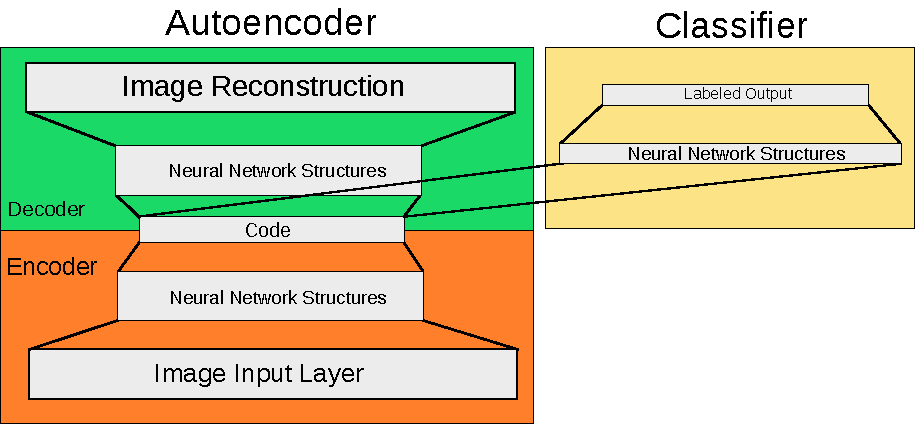
\includegraphics[width=0.5\textwidth]{illustrations/network_01.pdf}
 \captionof{figure}{General structure of the proposed network. Each rectangle
 represents many layers of neurons and the thin lines represent connections between layers.}
\end{figure}

Facial Action Unit detection FAU \cite{Corneanu2016} is chosen in this work due
to it's popularity and available benchmarks.
The Facial Action Coding System (FACS) developed by Ekman and Friesen,
provides a systematic way to study any kind of facial expression,
by representing them as a combination of individual facial muscle actions
known as Action Units (AU). Automating the process of detecting AUs is difficult
because they have non-linear interactions and often occur in very low intensities.

Deep learning is emerging as a powerful tool in modelling a wide range of patterns
in data, it has been applied to the problem of FAU a number of times and achieved
good classification rates. One complication which arises when using Deep Neural
Networks DNNs to classify AUs is that many frames are unlabelled (have neutral expressions)
and hence the standard supervised DNN do not make good use of this information.
This project aims to investigate how an autoencoder could be combined with the
already established deep learning methods related to FAU in order to improve the performance
of these techniques and better leverage unlabelled data. This unlabelled data may
come from within the standard AU datasets or from larger databases of faces.
The DISFA dataset is chosen for initial experiments.
\section{Potential Applications}
\section{Contributions}
\section{Thesis Outline}
\chapter{Background}

\section{Databases for FAU estimation}
Relevant for this work is a awareness of datasets which exist and may be useful
for experiments. Here is a list of some which should be used in order to allow
this project to be comparable to work in the literature:

\begin{itemize}
    \item CK+ \cite{Lucey2010} containing 123 subjects recorded with faces in strictly front positions.
    \item The DISFA database \cite{disfa}, which contains only 27 people whose spontaneous
          facial expressions were captured in controlled recording conditions.
    \item FERA 2015 BP4D-Spontaneous Dataset \cite{Valstar}:
          It consists of 41 subjects and 34 AUs, and the subjects were young adults who
          spontaneously generated emotional responses to stimulus tasks.
\end{itemize}

This is just a small selection, however is it representative of the types of
datasets available. Each frame of the videos has a label which describes which AUs are
present and their intensity. Hence two distinct problems can be tackled here, intensity
estimation and classification, this work follows the classification route however
intensity estimation should also be possible with a few minor modifications.

A key challenge with these datasets is that they often have very unbalanced and
sparse labels as shown in figure \ref{disfastats}. This calls for methods
to balance training samples with respect to this imbalance and is the
motivation for using some unsupervised learning techniques, in order to extract information
from the unlabelled data.

A further two datasets are the TFD and SEMAINE, these do not contain AUs but often crop up in the
literature:
\begin{itemize}
     \item TFD \cite{tfd} Toronto Face Dataset
     \item The SEMAINE \cite{semaine} corpus which contains recordings
           of people interacting with a Sensitive Artificial Listener (SAL) in controlled conditions.
\end{itemize}

\section{The DISFA dataset} \label{disfa_list}
The Denver Intensity of Spontaneous Facial Action Dataset (DISFA)
Of central interest to the project is the DISFA dataset \cite{disfa}, it is a set
of videos of people watching 9 short clips from youtube which try to


 it has 27 subjects with 12 AUs.
Each frame in each subject video has a label which says how much of each AU is present on
a scale of 0-5, the distribution of intensities is shown in table \ref{compau}.

A challenge of the DISFA dataset is that it has many frames which are unlabelled, this is demonstrated
per subject in figure \ref{disfastats}. Many of the subjects have over 40\% of their frames unlabelled
, one outlier has over 75\% unlabelled.

\begin{table}[h!]
\centering

\begin{tabular}{lllllll}
\hline
Intensity & 0      & 1     & 2     & 3     & 4    & 5    \\ \hline
AU1       & 112286 & 2272  & 1749  & 2809  & 1393 & 555  \\
AU2       & 99165  & 1720  & 934   & 3505  & 836  & 369  \\
AU4       & 106160 & 4661  & 7636  & 6586  & 4328 & 1383 \\
AU5       & 99015  & 1579  & 719   & 293   & 104  & 34   \\
AU6       & 106425 & 9157  & 5986  & 3599  & 601  & 141  \\
AU9       & 99458  & 1659  & 2035  & 3045  & 316  & 77   \\
AU12      & 99987  & 13943 & 6869  & 7233  & 2550 & 172  \\
AU15      & 108358 & 5180  & 1618  & 1017  & 47   & 0    \\
AU17      & 117824 & 6342  & 4184  & 2281  & 112  & 11   \\
AU20      & 121377 & 1591  & 1608  & 1305  & 28   & 0    \\
AU25      & 84721  & 9805  & 13935 & 15674 & 5580 & 1039 \\
AU26      & 105778 & 13443 & 7473  & 3529  & 314  & 217  \\ \hline
\end{tabular}
\caption{A comparison of the number of occurrences of each intensity for each AU in the DISFA dataset} \label{compau}
\end{table}


\begin{figure}[h!]
  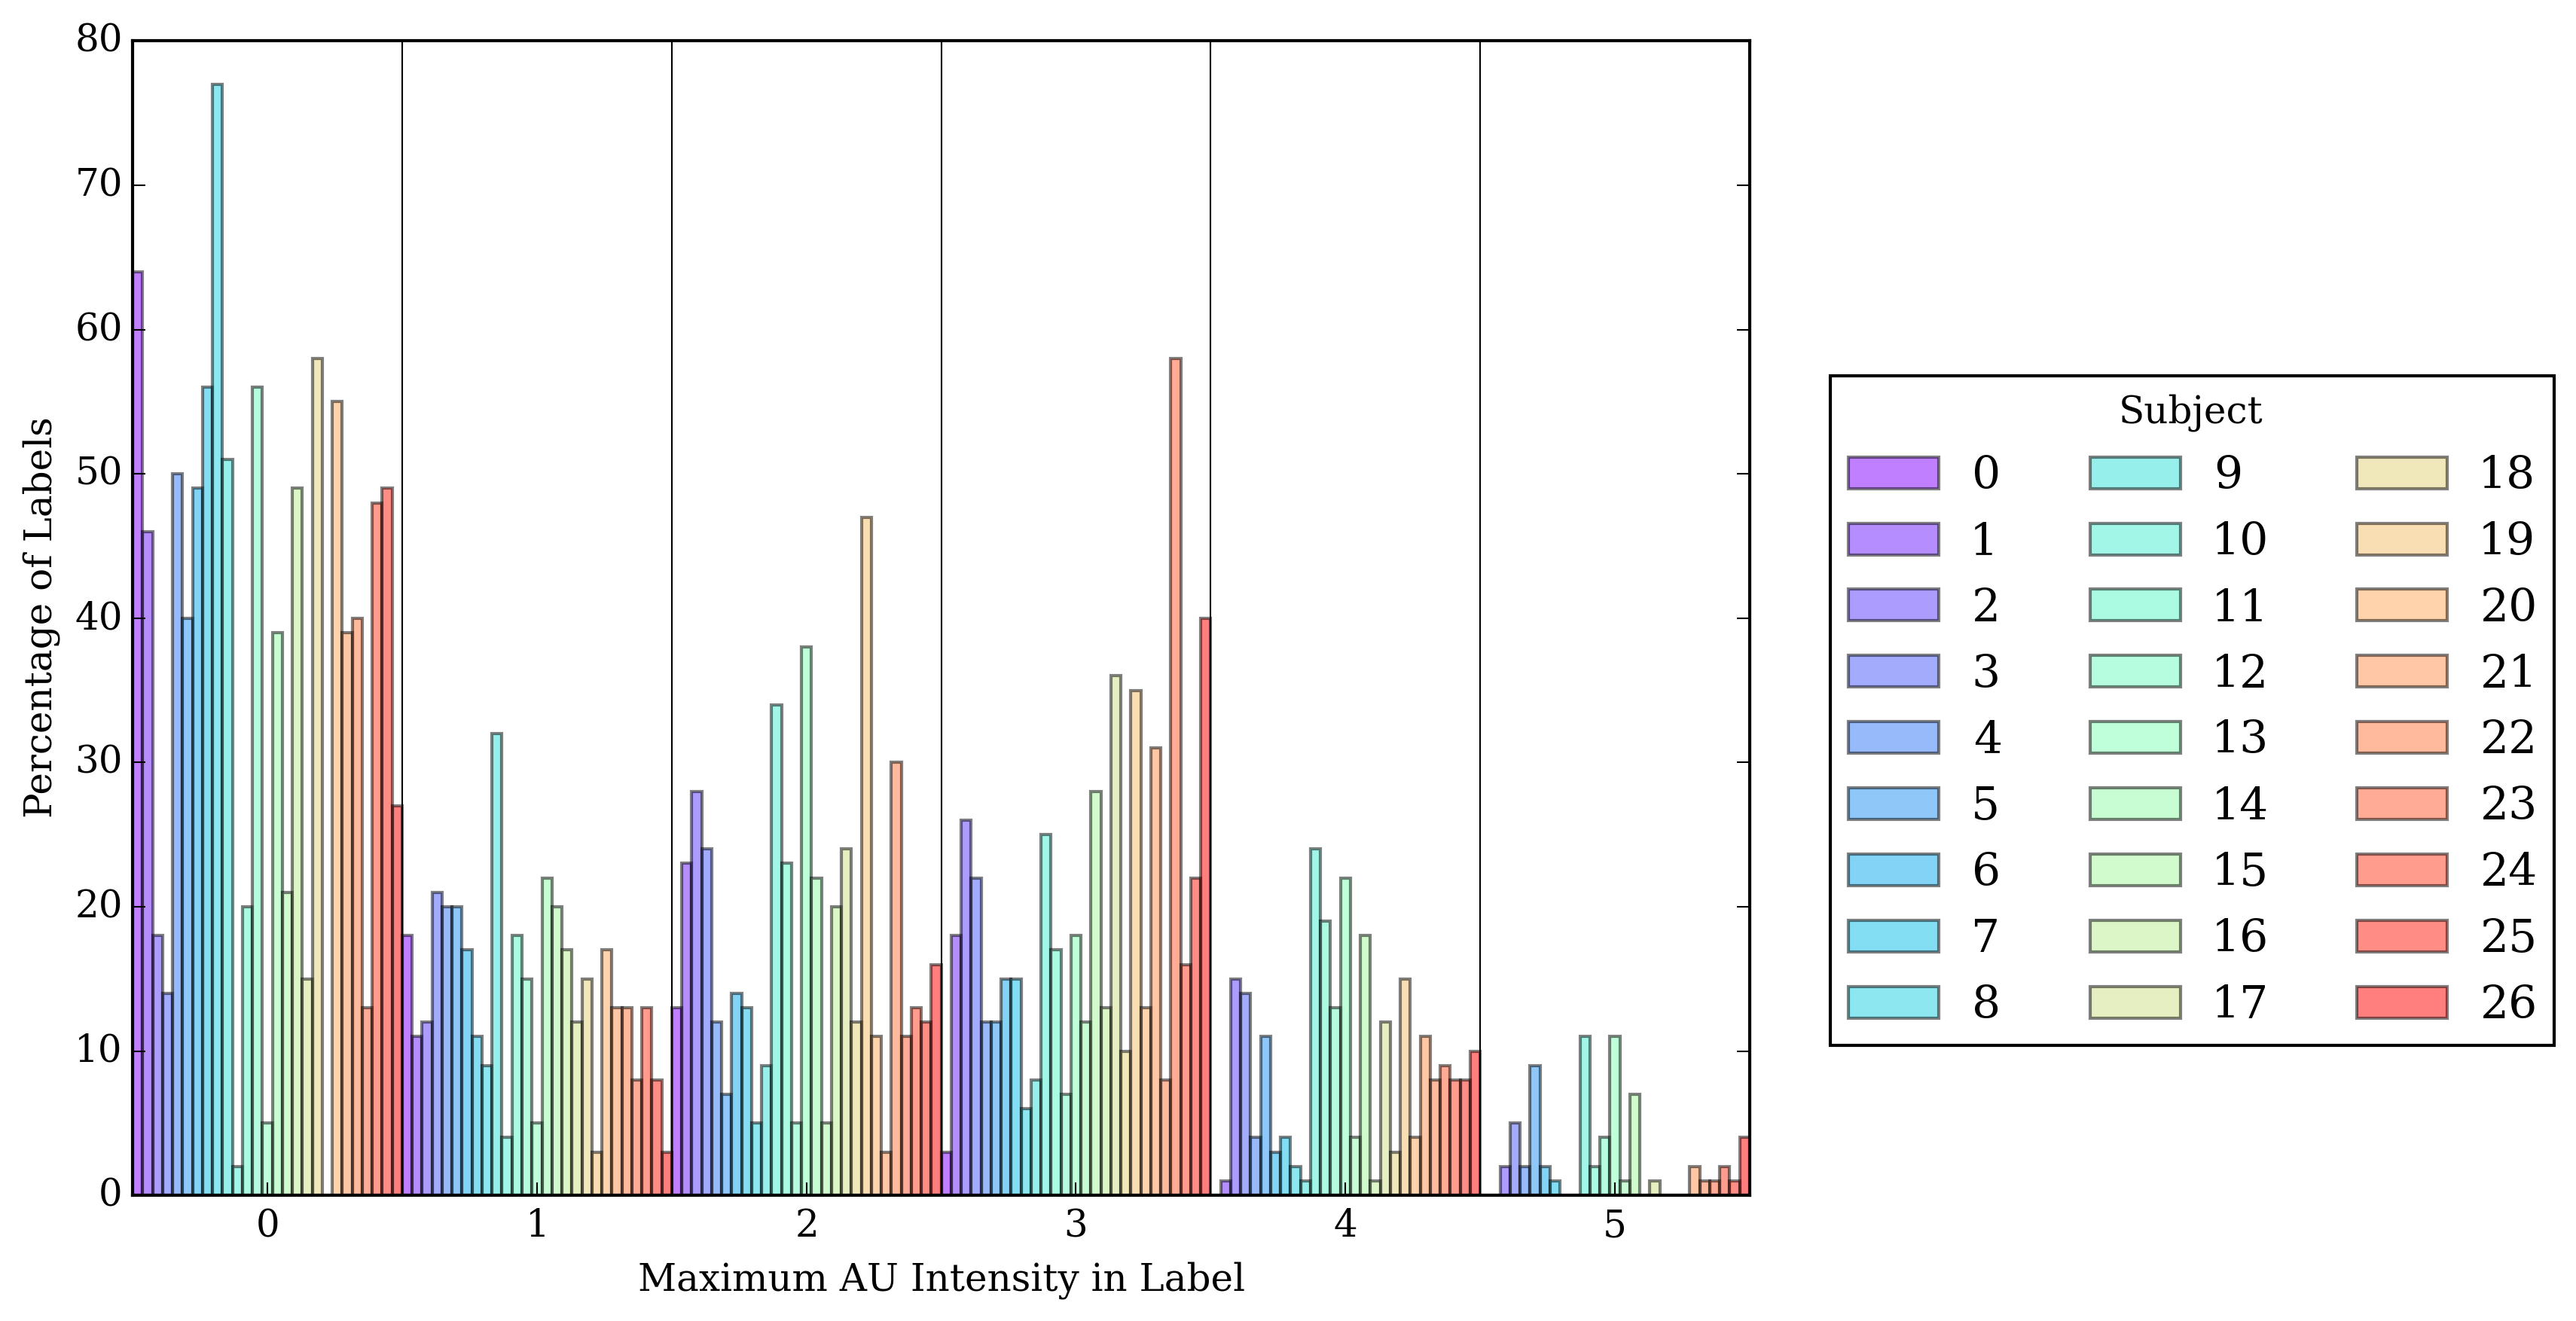
\includegraphics[width=\textwidth]{../graphs/maximum_label_intensity_disfa.pdf}
  \caption{DISFA dataset: This graph shows what the maximum value in each label is in the DISFA dataset per subject. This
  is done to illustrate the number of labels which contain absolutely no information.}\label{disfastats}
\end{figure}
\newpage

\section{Deep learning approaches to FAU detection}
It has been shown that deep neural networks containing convolutional, max pooling,
dropout and fully connected layers can effectively learn how to classify AUs in
a selection of datasets \cite{Gudi2015,Ghosh2015,dodeeplearn}. These
works only include networks which ignore the temporal structure of the data,
other architectures do incorporate this \cite{emonet,Jaiswal2016}.


%
%
%






\subsection*{Comparison of networks in Table \ref{compnet}}
Network \cite{Ghosh2015} (Ghosh et al.) was trained on CK+, DISFA and BP4D datasets.
A key result of this paper was that they achieved good generalisation between datasets
with classifications accuracies between 60\% and 80\% for these generalisation experiments.
A feature particular to this network was that after the softmax layer, which assigns probabilities
to each AU it uses QDA (Quadratic Discriminant Analysis) \cite{precogbook} to
make predictions about whether AUs are present. A point of interest is also that
mean face normalisation is done per subject and then all for all subjects.

Network \cite{Gudi2015} (Amogh Gudi et al.) was trained on BP4D and SEMAINE
datasets achieving an average F1 score of 0.52 and 0.34 respectively. This paper
uses minimal preprocessing hence is a good example of how CNNs can learn features
with little feature engineering.

Network \cite{dodeeplearn} (Pooya Khorrami et al.) was trained on TFD and CK+,
this got average accuracies of 89.9\% and 98.3\% respectively in detecting emotions. This
is therefore not directly comparable, but they do explore connecting it with AUs.
An interesting point about this work is that they could stimulate activations in the convolutional
layers and directly see that the network had learned different facial actions demonstrating the
power of these networks.

Network \cite{Jaiswal2016} (Shashank Jaiswal et al.) was trained on SEMAINE and
BP4D achieving an overall weighted F1 score of 0.54. Which is on average higher
than network \cite{Gudi2015} as claimed in the paper. This paper includes a lot more
prior knowledge than the others, firstly it uses a BLSTM to incorporate temporal structure
and it defines multiple input streams from each facial region, allowing the convolutional
filters to become more specialised. This is the only paper where they say they use
two outputs for each AU so that the softmax creates a probability distribution for
each AU and not for all of them at once.

It should be noted that it is difficult to compare the performance between these
networks as they all use different evaluation scores as shown in table \ref{compscore}.

\begin{table}[h!]
\centering
{\footnotesize
\begin{tabular}{|lllllllll|}
\hline
Network                      & \multicolumn{2}{c}{Ghosh et. al\cite{Ghosh2015}}                         & \multicolumn{2}{c}{Gudi et. al.\cite{Gudi2015}}                            & \multicolumn{2}{c}{Khorrami et. al.\cite{dodeeplearn}}                          & \multicolumn{2}{c|}{Jaiswal et. al.\cite{Jaiswal2016}}   \\ \hline
\multicolumn{1}{|l|}{Element} & Type     & \multicolumn{1}{l|}{Dimensions}                    & Type     & \multicolumn{1}{l|}{Dimensions}                      & Type          & \multicolumn{1}{l|}{Dimensions}                  & Type      & Dimensions                     \\ \hline
\multicolumn{1}{|l|}{x}       &          & \multicolumn{1}{l|}{$40\times40\times1$}           &          & \multicolumn{1}{l|}{$48\times 48\times1$}            &               & \multicolumn{1}{l|}{$96\times96\times1$}         &           & $?\times?\times1$              \\ \hline
\multicolumn{1}{|l|}{$L_1$}   & conv 1   & \multicolumn{1}{l|}{$12\times 12\times1\times 70$} & conv 1   & \multicolumn{1}{l|}{$5\times 5\times1\times64$}      & conv 1        & \multicolumn{1}{l|}{$5\times5\times1\times64$}   & conv 1*   & $5\times5\times(2n+1)\times32$ \\
\multicolumn{1}{|l|}{$y_1$}   &          & \multicolumn{1}{l|}{$29\times29\times70$}          &          & \multicolumn{1}{l|}{$44\times44\times64$}            &               & \multicolumn{1}{l|}{$92\times92\times64$}        &           & $?\times?\times32$             \\ \hline
\multicolumn{1}{|l|}{$L_2$}   & max pool & \multicolumn{1}{l|}{$2\times 2$}                   & max pool & \multicolumn{1}{l|}{$3\times3$ (stride 2)}           & max pool      & \multicolumn{1}{l|}{$2\times2$}                  & max pool*  & $3\times3$                    \\
\multicolumn{1}{|l|}{$y_2$}   &          & \multicolumn{1}{l|}{$15\times15\times 70$}         &          & \multicolumn{1}{l|}{$22\times 22\times64$}           &               & \multicolumn{1}{l|}{$46\times46\times64$}        &           & $?\times?\times32$             \\ \hline
\multicolumn{1}{|l|}{$L_3$}   & conv 2   & \multicolumn{1}{l|}{$4\times 4\times70\times 10$}  & conv 2   & \multicolumn{1}{l|}{$5 \times 5 \times 64\times64$}  & conv 2        & \multicolumn{1}{l|}{$5\times5\times64\times128$} & conv 2    & $5\times5\times32\times64$     \\
\multicolumn{1}{|l|}{$y_3$}   &          & \multicolumn{1}{l|}{$12\times 12 \times 10$}       &          & \multicolumn{1}{l|}{$18 \times 18\times64$}          &               & \multicolumn{1}{l|}{$42\times42\times128$}       &           & $?\times?\times64$             \\ \hline
\multicolumn{1}{|l|}{$L_4$}   & max pool & \multicolumn{1}{l|}{$2\times 2$}                   & conv 3   & \multicolumn{1}{l|}{$4\times 4 \times64 \times 128$} & max pool      & \multicolumn{1}{l|}{$2\times2$}                  & conv 3    & $5\times5\times64\times64$     \\
\multicolumn{1}{|l|}{$y_4$}   &          & \multicolumn{1}{l|}{$6\times 6 \times 12$}         &          & \multicolumn{1}{l|}{$15\times15\times128$}           &               & \multicolumn{1}{l|}{$21\times21\times128$}       &           & $?\times?\times64$             \\ \hline
\multicolumn{1}{|l|}{$L_5$}   & fc       & \multicolumn{1}{l|}{$500$}                         & fc       & \multicolumn{1}{l|}{$3072$}                          & conv 3        & \multicolumn{1}{l|}{$5\times5\times1\times256$}  & conv 3    & $4\times4\times64\times128$    \\
\multicolumn{1}{|l|}{$y_5$}   &          & \multicolumn{1}{l|}{$500$}                         &          & \multicolumn{1}{l|}{$3072$}                          &               & \multicolumn{1}{l|}{$17\times17\times256$}       &           & $?\times?\times128$            \\ \hline
\multicolumn{1}{|l|}{$L_6$}   & fc       & \multicolumn{1}{l|}{$100$}                         & softmax  & \multicolumn{1}{l|}{$12$}                            & quadrant pool & \multicolumn{1}{l|}{}                            & fc        & $3072$                         \\
\multicolumn{1}{|l|}{$y_6$}   &          & \multicolumn{1}{l|}{$100$}                         &          & \multicolumn{1}{l|}{$12$}                            &               & \multicolumn{1}{l|}{$4\times4\times256$}         &           & $3072$                         \\ \hline
\multicolumn{1}{|l|}{$L_7$}   & softmax  & \multicolumn{1}{l|}{$12$}                          &          & \multicolumn{1}{l|}{}                                & fc            & \multicolumn{1}{l|}{$300$}                       & softmax   & $2N_{C}$                       \\
\multicolumn{1}{|l|}{$y_7$}   &          & \multicolumn{1}{l|}{$12$}                          &          & \multicolumn{1}{l|}{}                                &               & \multicolumn{1}{l|}{$300$}                       &           & $2N_{C}$                       \\ \hline
\multicolumn{1}{|l|}{$L_8$}   & QDA      & \multicolumn{1}{l|}{}                              &          & \multicolumn{1}{l|}{}                                & softmax       & \multicolumn{1}{l|}{$8$}                         & BLSTM     &                                \\
\multicolumn{1}{|l|}{$y_8$}   &          & \multicolumn{1}{l|}{}                              &          & \multicolumn{1}{l|}{}                                &               & \multicolumn{1}{l|}{$8$}                         &           &                                \\ \hline
\end{tabular}

\caption{A comparison of network architectures from the literature, all networks
use RELUs as their activation functions apart from in the final layer where it is
typical to use a softmax. $x$ denotes the input image, $L_i$ denotes the $i$th layer and $y_i$ denotes the output of the $i$th layer.
$N_{C}$ is the number of classes.
The question marks signify the dimensions of input images are variable as it depends on the input stream. fc is for fully connected and
conv is for convolutional layer. QDA is Quadratic Discriminant Analysis and BLSTM is for Bidirectional Long Short-Term Memory neural
networks.
\newline
*These layers are per input stream} \label{compnet}

}
\end{table}

\begin{table}[h!]
\centering

\begin{tabular}{lcccc}
\hline
Score    & \multicolumn{1}{l}{Ghosh et. al\cite{Ghosh2015}} & \multicolumn{1}{l}{Network Gudi2015} & \multicolumn{1}{l}{Gudi et. al.\cite{Gudi2015}} & \multicolumn{1}{l}{Khorrami et. al.\cite{dodeeplearn}} \\ \hline
Accuracy & \checkmark                            &                                      &                                         & \checkmark                              \\
F1       &                                       & \checkmark                           & \checkmark                              &                                         \\
AUC      &                                       &                                      &                                         &                                         \\
2AFC     & \checkmark                            &                                      & \checkmark                              &                                         \\ \hline
\end{tabular}
\caption{A comparison of which evaluation methods were used in a selection of papers.} \label{compscore}
\end{table}

\begin{table}[h!]
\centering

\begin{tabular}{lcccc}
\hline
Dataset  & \multicolumn{1}{l}{Ghosh et. al\cite{Ghosh2015}} & \multicolumn{1}{l}{Network Gudi2015} & \multicolumn{1}{l}{Gudi et. al.\cite{Gudi2015}} & \multicolumn{1}{l}{Khorrami et. al.\cite{dodeeplearn}} \\ \hline
CK+      & \checkmark                            &                                      &                                         & \checkmark                              \\
DISFA    & \checkmark                            &                                      &                                         &                                         \\
SEMAINE* &                                       & \checkmark                           & \checkmark                              &                                         \\
BP4D*    & \checkmark                            & \checkmark                           & \checkmark                              &                                         \\
TFD      &                                       &                                      &                                         & \checkmark                              \\ \hline
\end{tabular}
\caption{A comparison of which datasets were used in a selection of papers.} \label{compdat}
\end{table}


%
%
%
\chapter{Deep Learning}
\section{Introduction}
\section{Model Componenents}
\subsection{Artificial Neural Networks}
An artificial neuron is a function which takes in a vector of inputs, computes their
weighted sum and applies a non-linearity as follows:
\begin{equation}
    a(\mathbf{x}) = \sigma \left ( \sum_{i=1}^N w_ix_i + b \right )
\end{equation}
Here $\sigma$ is a scalar function, $w_i$ is a scalar weight and $b$ is its bias. $N$ is the size of the input and weight vector.
These neurons can be combined into layered networks to construct artificial neural networks.
The weights $w$ can then be rewritten as matrices $\mathbf{W}$ which define how
activations from one layer are transferred to the next\footnote{Note: when a vector
is put into a scalar function it is assumed that it acts on each element of
the vector. The only exception is with the softmax.}.
\begin{equation}
    \mathbf{a}(\mathbf{x}) = \mathbf{\sigma} \left ( \mathbf{W}\mathbf{x} + \mathbf{b} \right ) \label{eq:softmax}
\end{equation}

Popular activation functions include:
\begin{multicols}{2}


\begin{equation}
\text{The sigmoid:}\quad
  \sigma (x) = \frac{1}{1-e^{-x}} \label{eq:sigmoid}
\end{equation}


\begin{equation}
\text{The ReLU:}\quad
\sigma(x) =
\begin{cases}
      x & x\geq 0 \\
      0 & x < 0
   \end{cases}
\end{equation}


\begin{equation}
\text{Hyperbolic tan:}\quad
    \sigma(x)=\frac{e^x - e^{-x}}{e^x + e^{-x}}
\end{equation}


\begin{equation}
\text{The softmax:}\quad
  \sigma(\mathbf{x})_j = \frac{e^{x_j}}{\sum_i e^{x_i}}
\end{equation}


\end{multicols}

\begin{figure} \label{disfagraph}
    \center
  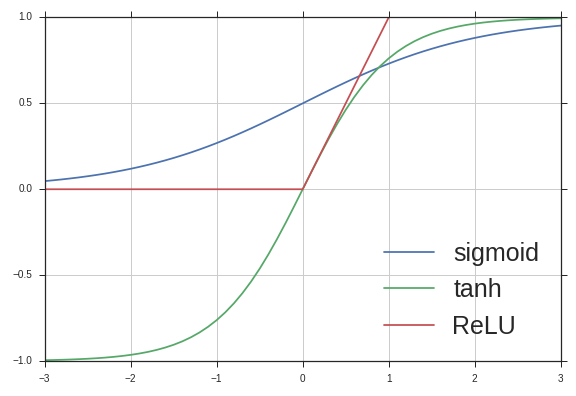
\includegraphics[width=.5\textwidth]{../graphs/actfuncs.pdf}
  \caption{Comparison of common activation functions for neural networks}
\end{figure}



An $N$ layer network can
then be thought of as a function with a recursive structure (these are also known as fully connected layers):
\begin{equation}
    \mathbf{y} = \mathbf{a}_{N}(\mathbf{a}_{l-1}(...\mathbf{a}_1(\mathbf{x})...))
\end{equation}
Now assuming there exists a set of $\tilde{\mathbf{x}}$ and $\tilde{\mathbf{y}}$ which make
up a training data set, these could be sets of images and labels, then a cost function
to optimise can be defined:
\begin{equation}
    J(\tilde{\mathbf{x}},\tilde{\mathbf{y}}) = \frac{1}{N}\left |\mathbf{y}(\tilde{\mathbf{x}})-\tilde{\mathbf{y}}\right | ^2
\end{equation}
this is called the least mean squared error, another popular cost function is
the cross entropy:
\begin{equation}
    J(\tilde{\mathbf{x}},\tilde{\mathbf{y}}) = -\frac{1}{N}\tilde{\mathbf{y}}\cdot\log(\mathbf{y}(\tilde{\mathbf{x}}))
\end{equation}

The derivative of these cost functions can then be computed in order to minimise it.
The simplest way is to do this is per training example, however stochastic gradient
descent\cite{Amari1993} has emerged as a superior method. Simply put it computes the gradient with respect
to many randomly drawn samples, it has the advantage of following a smoother path
towards the local minimum.
\subsection{Convolutional Layers}
A convolutional layer is a generalisation of simple fully connected layers described
above. It consists of a set of $K$ filters of size $m\times m$, which are applied to the input to produce
a set of $K$ outputs. The filters are applied with a 2D convolution.


To describe them, firstly assume that any vector described in the previous section
can also be rewritten as a matrix, i.e $\mathbf{x} \in \mathbb{R}^{n}
\rightarrow \mathbf{x} \in \mathbb{R}^{N \times M} \quad NM=n$, in practice this is made
easy by using numbers which factorise well.

Then the following equation describes the output of a convolutional layer:
\begin{equation} \label{CNN}
    \mathbf{a}(\mathbf{x})_{ijk} = \sigma \left ( \sum_{a=0}^{m-1}\sum_{b=0}^{m-1}(w_{abk}x_{(i+a)(j+b)k}) + b_k \right )
\end{equation}
Here $i,j$  denote row, column indices for the matrix (image) $\mathbf{x}$, $k$ is the filter index, $w_{abk}$
gives the filter element and $b_k$ is the bias for that filter. This is done for all $K$ filters.

One issue is how to deal with indices which are out of bounds, SAME padding can be used which sets out of bounds
elements to zero and so preserves the image size or VALID can be used, this keeps the filter within the bounds of the
image and hence the output is of a smaller dimension. Lastly a stride greater than 1 can be incorporated into equation
\ref{CNN} meaning that $\mathbf{a}$ is only computed for a fraction of indices $i,j$.
% \begin{equation}
% 	C : \mathbb{R}^{n\times m \times p \times l} \rightarrow \mathbb{R}^{N\times M \times l \times K}
% \end{equation}
%con%
\subsection{Max Pooling Layers}
A max pooling layer simply splits its input into a set of sections and extracts
the highest value from each. It is a simple but effective method to down sample
an image, it helps to keep the computational overhead of these algorithms
down. However a recent trend \cite{Springenberg2015} has emerged where max pooling
layers are not used, instead a convolutional layer with a large stride accomplishes
the same amount of down-sampling.
\subsection{Dropout Layers}
A layer with dropout applied to it randomly turns neurons off, making it more
difficult for the network to overfit data. There is a dropout probability
which determines how often neurons are disabled, it is typically under 20\%
\subsection{Autoencoders}
An autoencoder is at its bare minimum a artificial neural network which tries
to reproduce its input as accurately as possible. So the cost function for the
least mean squared error becomes:

\begin{equation}
    J(\tilde{\mathbf{x}},\tilde{\mathbf{y}}) = \frac{1}{N}\left |\mathbf{y}(\tilde{\mathbf{x}})-\tilde{\mathbf{x}}\right | ^2
\end{equation}

Constraints are
placed on the network so that it has to learn to compress the input, the following
are popular constraints that may be used:
\begin{itemize}
    \item Few neurons in the hidden layers
    \item Sparsity: the average activation of the neurons can be kept under a
    threshold, typically a small value close to zero \cite{autong}
    \item Noise may be added to the input, this makes the network more likely
    to learn general features.
\end{itemize}
Lastly there are Variational Autoencoders which combine ideas from Bayesian inference
to create networks which can not only reconstruct their input but also act as a
distribution which can be sampled from, allowing for the generation of new samples \cite{Kingma2013}.

\subsection{Stacked Autoencoder}

A stacked autoencoder is typically used for pre-training a network for a classification task.
Instead of training the whole structure at once, each layer is trained as the last hidden
layer of some temporary autoencoder. It has been shown that this can improve classification performance \cite{stacks}.


\subsection{Convolutional Autoencoder}
A convolutional autoencoder works in the same way as a standard autoencoder, however
undoing the max pooling presents a problem, as a max pooling layer throws away
information, its inverse will never be exact. The following strategies have been
used with success:
\begin{itemize}
    \item Replacing each entry with an $n \times n$ matrix filled with the original
    entry.
    \item Replacing each entry with an  $n\times n$  matrix with
    the original entry in the upper left and the other squares set to 0. \cite{Dosovitskiy2015}
\end{itemize}

Other than that all other elements have very straightforward inverses and hence
a convolutional autoencoder can be constructed.

\section{Model Evaluation}
With any kind of classification model it is crucial to be able to evaluate its
performance, in a standard and reproducible way. For the problem of classifying
AUs the simplest case is to split the problem into a set of $n_C$ decision problems
where $n_C$ is the number of distinct classes. Now the problem is reduced to
evaluating the performance of a binary classifier. Finding the confusion matrix is
the first step in such a problem. For a binary problem it is defined as follows:
\begin{equation}
C =
\begin{pmatrix}
TP & FN\\
FP & TN
\end{pmatrix}
\end{equation}
Where $TP$ is the number of true positives, $FN$ is the number of false negatives
, $FP$ is the number of true positives and $TN$ is the number of true negatives.
In a perfect classification, this matrix would have $FP=FN=0$, however this is rare
and we can define quantities to measure how close to this ideal we are. Note we
only define the binary case here, the more general confusion matrix for multiple
classes can easily be defined but is not relevant here.
\begin{equation}
\text{Recall} = \frac{TP}{TP+FN}
\end{equation}
\begin{equation}
\text{Precision} = \frac{TP}{TP+FP}
\end{equation}
\begin{equation}
\text{F1} = 2 \cdot \frac{\text{Recall} \cdot \text{Precision}}{\text{Recall} + \text{Precision}}
\end{equation}

Hence recall is decreased by false negatives, i.e not being able to recall the class
when presented with it. Precision is decreased by false positives i.e stating the class
is present when it is not. Both measures describe a different aspect of the accruacy and so the F1 is the
harmonic mean between these two, it is the quantity this report will seek to maximise and use to compare
results with the literature.

Another useful measure is the area under the Receiver operating characteristic (ROC) curve.
As neural networks output a number between 0 and 1, a threshold must be chosen to signify
when the network declares a class present. By varying this threshold a series of true positive and false positive rate points
can be generated, this is the ROC curve. The area under this is ideally 1 and in the worst case 0, hence this is
another measure of classification accuracy that is invariant to the chosen threshold.

\chapter{Implementation}
\section{Project Structure}
\section{Deep Learning Framework}
Tensorflow \cite{tensorflow} was chosen as the deep learning framework for this
project. Many others exist, some advantages that tensorflow has over its rivals
includes platform independence, distributed computing and inbuilt visualisation
of network topology and parameters over time. As most other frameworks it uses python
to define it's computations and also includes a C++ interface.


\chapter{Preprocessing Labeled Faces}
\section{Introduction}
It is typical to apply some sort of preprocessing methods to any data fed into
a neural network.Using previous work of Sebastian Kaltwang (See acknowledgements) the
DISFA data set has frames of size $118 \times 118$ with pixel values integers between
0 and 255. This section defines and visualizes 3 different ways of normalisiing and scaling
this data.



\begin{equation}
  {\bf P}({\bf x},i) = {\bf x'}_i
\end{equation}
\begin{equation}
  {\bf P}({\bf x},i,s) = {\bf x'}_{si}
\end{equation}
\begin{figure}[!h]
\centering
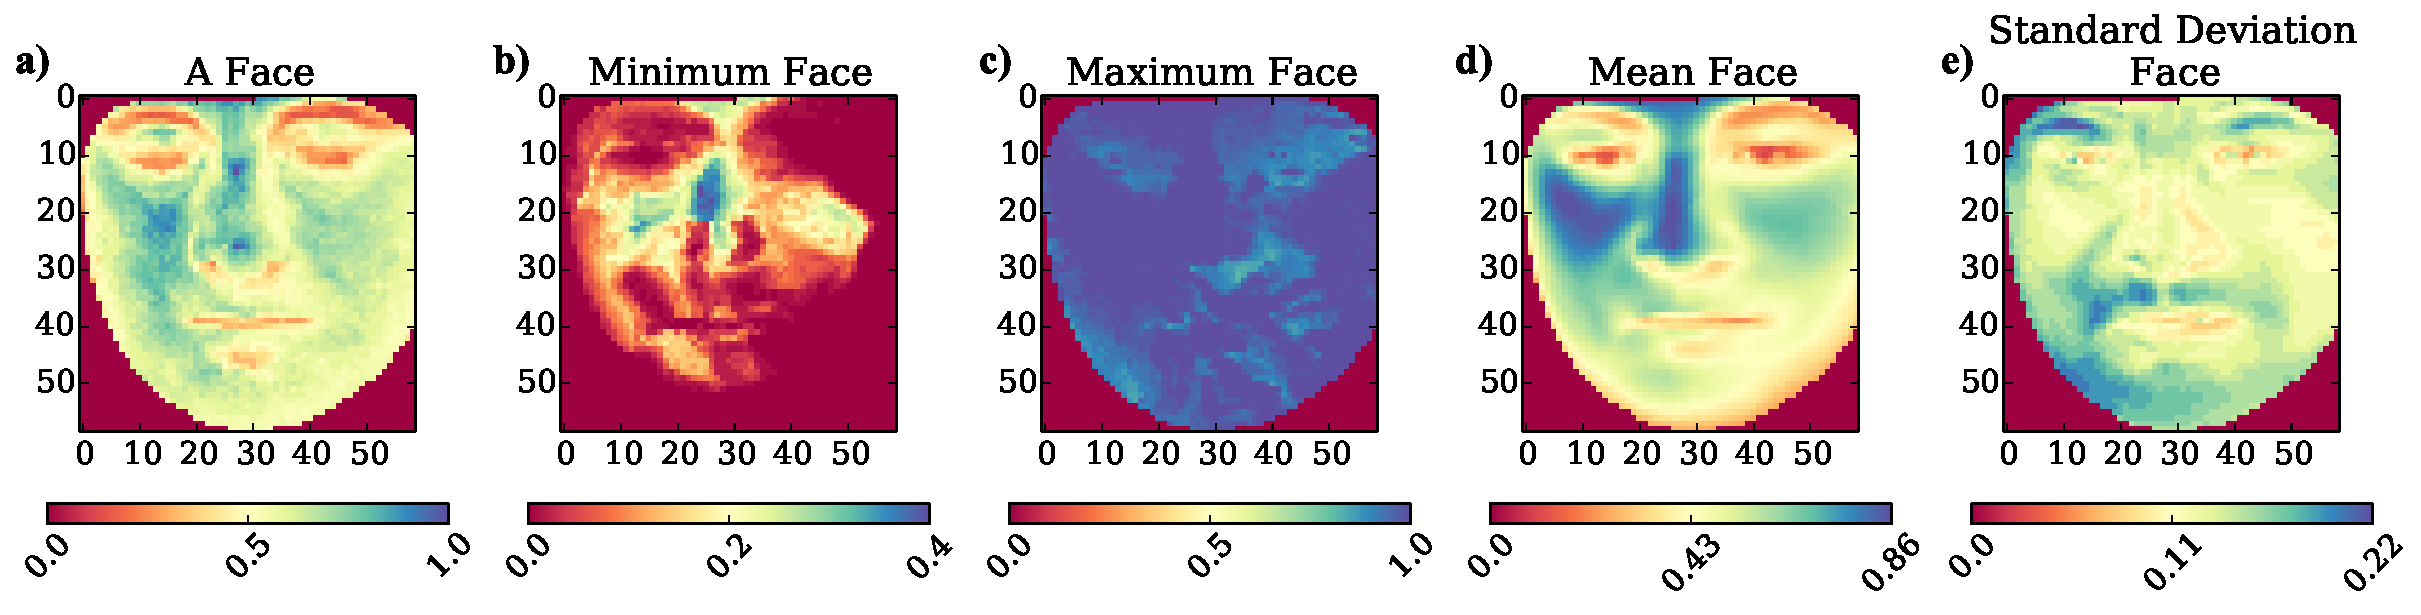
\includegraphics[width =\hsize]{figures/faces.pdf}
\caption{hello}
\label{fig:simple}
\end{figure}

\begin{equation}
  {\bf P}({\bf x},i) = {\bf x'}_i
\end{equation}
\begin{equation}
  {\bf P}({\bf x},i,s) = {\bf x'}_{si}
\end{equation}
\begin{figure}[!h]
\centering
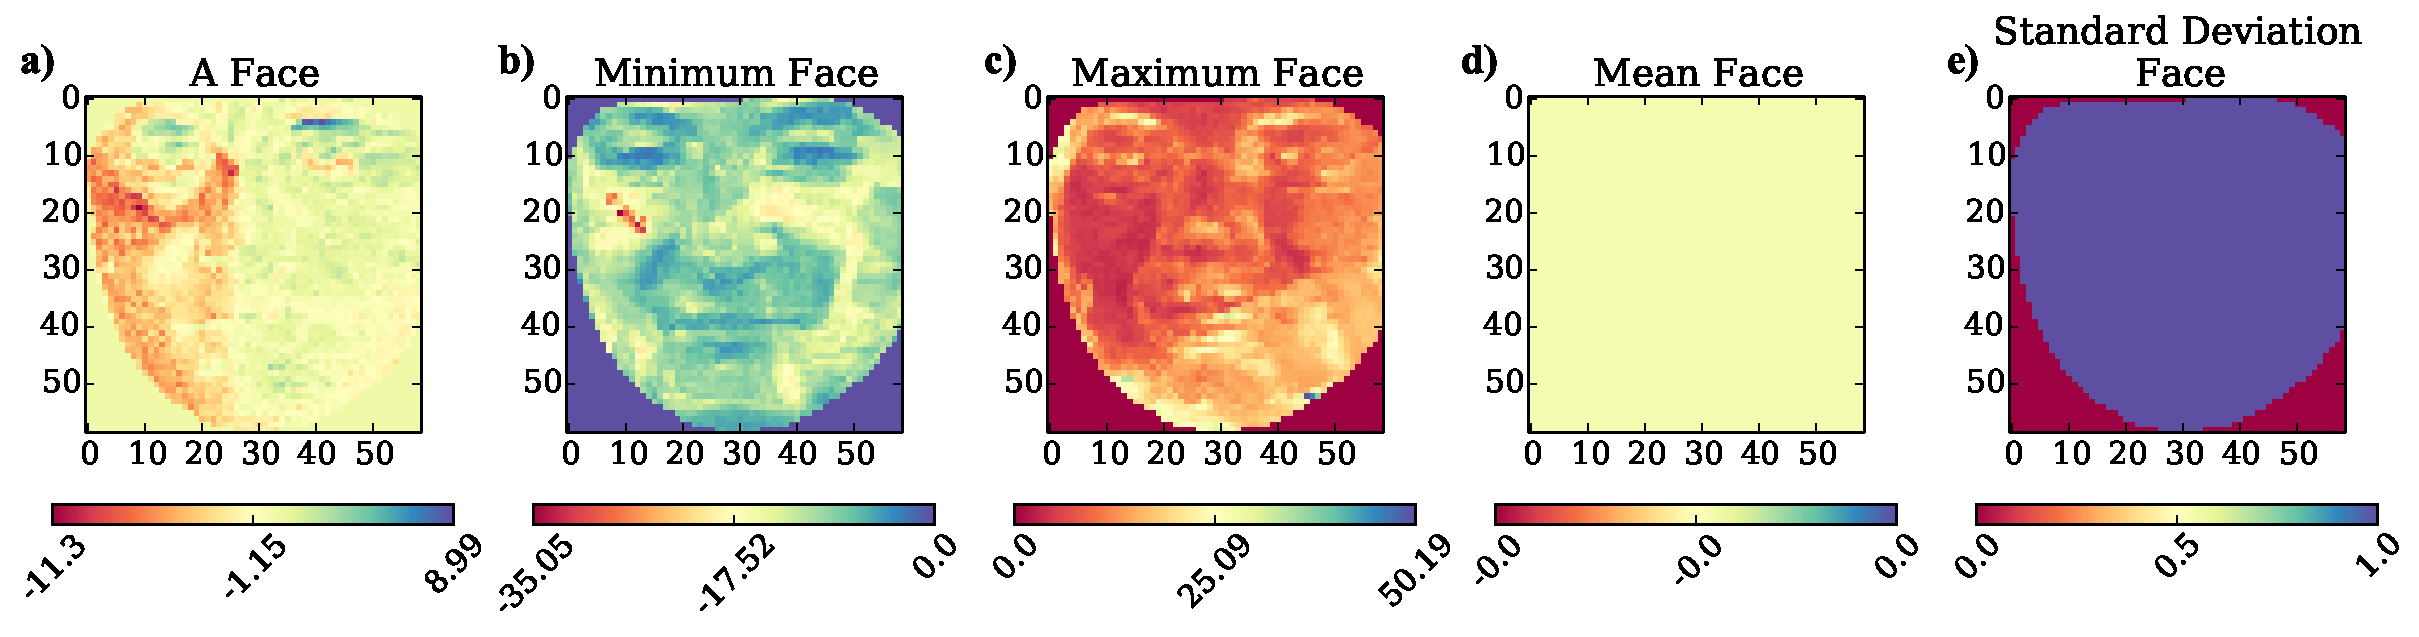
\includegraphics[width =\hsize]{figures/faces_per_subject_face.pdf}
\caption{hello}
\label{fig:simple}
\end{figure}

\section{Methods}
The preprocessing methods assume a dataset of a number of subjects
is described as a data structure of the form:
\begin{equation}
{\bf x} \in \mathbb{R}^{N\times X \times Y},\quad {\bf y} \in \mathbb{N}^{N\times F}
\end{equation}
Where $N$ is the number of images, $X$ is the width of the image, $Y$ is the height of the
image and $F$ is the number of AU's labeled. Furthermore in some cases an extra dimension
for subject may be added:
\begin{equation}
{\bf x} \in \mathbb{R}^{S\times N\times X \times Y},\quad {\bf y} \in \mathbb{N}^{S\times N\times F}
\end{equation}
Some subjects may have a slightly different number of frames and this is reflected
in the implementation but not in this section.

Each preprocessing method will be denoted by a function ${\bf P}$ defined as follows:


\subsection{Contrast Normalisation}

\begin{equation}
  {\bf P}({\bf x},i) = {\bf x'}_i
\end{equation}
\begin{equation}
  {\bf P}({\bf x},i,s) = {\bf x'}_{si}
\end{equation}
\begin{figure}[!h]
\centering
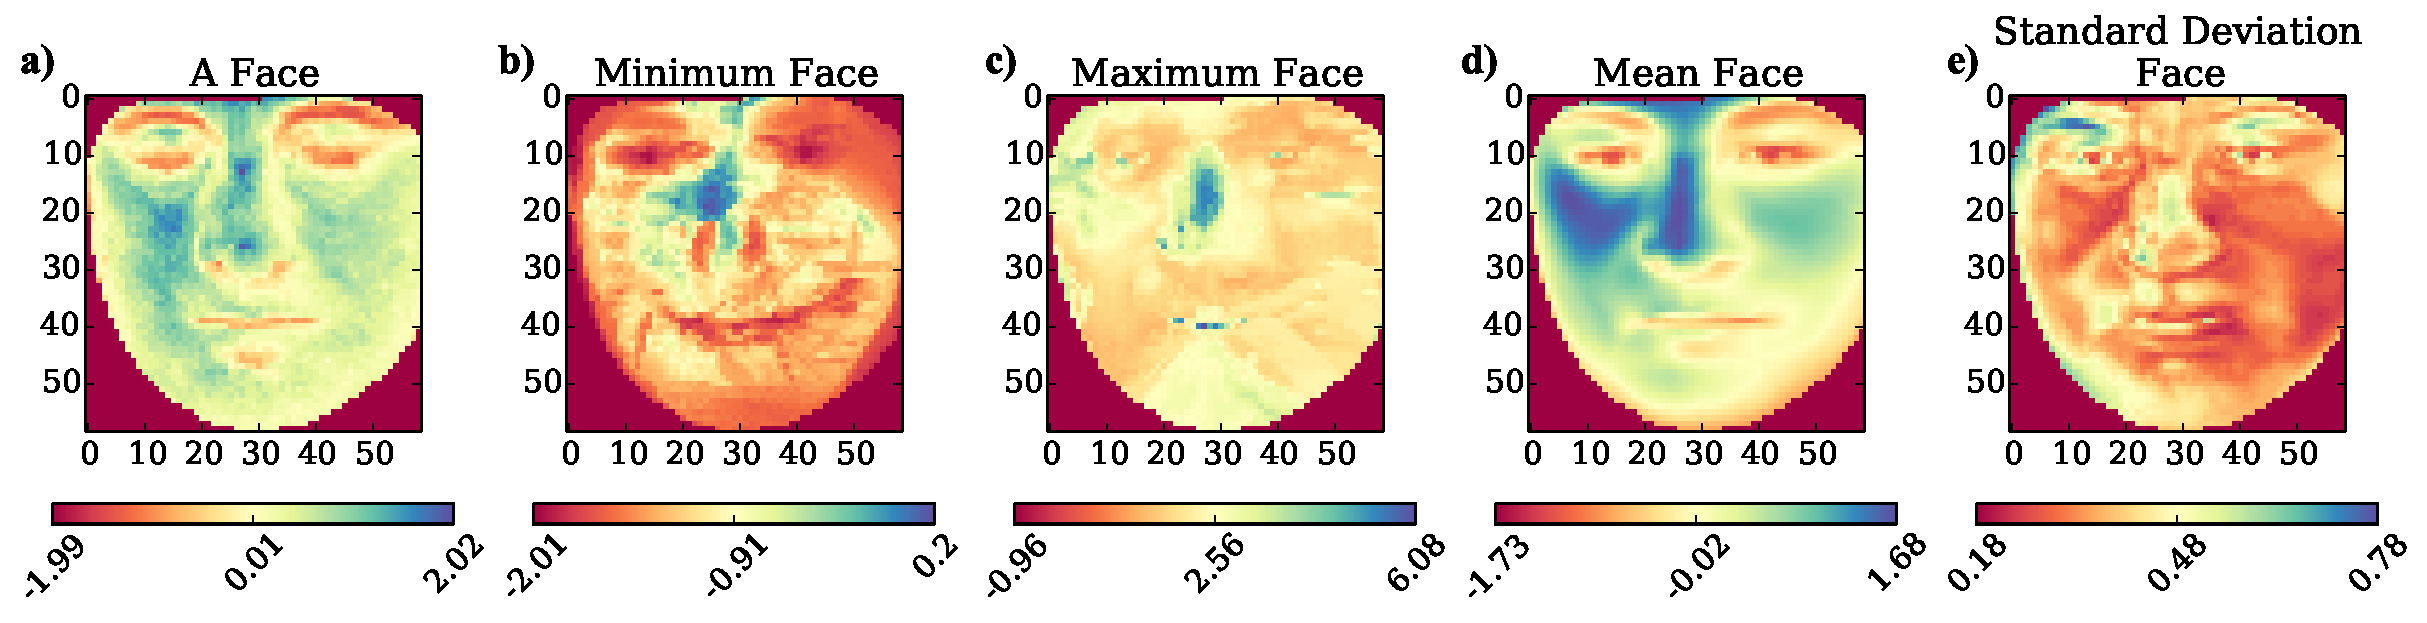
\includegraphics[width =\hsize]{figures/faces_contrast.pdf}
\caption{hello}
\label{fig:simple}
\end{figure}

For each image find the mean pixel value and standard deviation and then subtract the mean
and divide by the standard deviation. This standardises the amount of contrast in each image.
\begin{equation}
   P({\bf x},i)= ({\bf x}_{ijk} - \bar {\bf x}_{i})/\sigma ({\bf x}_{i}) = {\bf x}_{ijk}'
   \label{eq:con}
\end{equation}
Equation \ref{eq:con} shows this, a disadvantage of this normalisation is that it
has no regard of facial structures.
\subsection{Mean Face Normalisation}
Here the mean face and standard deviation face is subtracted and divided away from the
image, these faces might be per subject or per dataset, as shown:
\begin{equation}
  P({\bf x},i) =  ({\bf x}_{i} - \bar {\bf x})/\sigma ({\bf x}_{i})  = {\bf x}_{i}'
\end{equation}
\begin{equation}
  P_s({\bf x},s,i) = ({\bf x}_{si} - \bar {\bf x}_s)/\sigma ({\bf x}_{si})  = {\bf x}_{si}'
\end{equation}
The point of this normalisaiton is to enhance the intensity of any pixels which
are unusal, these pixels should hold most information about potential facial expressions.
\subsection{Range Scaling}
This normalisation stretches the data between -1 and 1, this contains no feature engineering
intution but is simply another type of normalsiation to try.
\begin{equation}
  r({\bf x})_{axis} = \max_{axis}({\bf x}) - \min_{axis}({\bf x})
\end{equation}
\begin{equation}
   P({\bf x},i) =
   \frac{{\bf x}_{i} - \frac{1}{2}\left ( \min_0({\bf x}) + \max_0({\bf x}) \right ) }{\frac{1}{2}r_0({\bf x})}
   = {\bf x}_{i}'
\end{equation}
\begin{equation}
   P_s({\bf x},i,s) =
   \frac{{\bf x}_{si} - \min_0({\bf x}_s) - \frac{1}{2}r_0({\bf x}_s) }{\frac{1}{2}r_0({\bf x}_s)}
   = {\bf x}_{si}'
\end{equation}


%%%%%%%%%%%%%%%%%%%%%%%%%%%%%%%%%%%%
\chapter{Modelling DISFA}
This chapter details the path followed in determining which network structures worked and
which did not. The most important metric for a network will be the Average ROC of the classifier
when applied to the un-seen validation set. The section will not be in chronological order of
experiment but in an order which puts fundamental ideas first.
\section{Joint classification}

Typical deep neural networks are used have to classify
one frame into only one category. The case with the DISFA dataset is different, we
would like to be able to classify the categories jointly,  putting one frame into more than
one AU category. Ideally the network would output a confidence score between 0 and 1
to signfy if an AU is present and we would calculate some optimum threshold value
(ideally this would be 0.5).

The following list details three possible solutions and table \ref{tab:softmax}
compares how they perform, using a small network which contains a convolutional layer, max pooling and
also an autoencoder branch (which is included only to be used as a relative performance measure).

\begin{itemize}
  \item {\bf Softmax Layer} - This is a traditional, fully connected layer with
                              a softmax activation function (see equation \ref{eq:softmax}).
                              The issue with this is that it provides a probability distribution over AUs
                              but the required quantity is a probability distribution for each AU.
  \item {\bf Sigmoid Layer} - This again is like the previous solution but instead each neuron gives a confidence
                              score between 0 and 1 for each AU with a sigmoid function (see equation \ref{eq:sigmoid}).
                              The issue with this however is that sigmoid
                              functions have vanishing gradients at large input values
                              hence training may become difficult.
  \item {\bf Binary Softmax Layers} - Here there is a two neuron softmax layer
                                      for each AU, this doubles the amount of weights
                                      but gives a probability over the presence and
                                      absence of each AU which is ideal.
\end{itemize}

The following table shows results from an experiment, to compare the above methods:

\begin{table}[!h] {\small
  \centering
  \begin{tabular}{lccc}
  \hline
  Final Layer   & Av. ROC &   Av. Best F1 &   Autoencoder Loss (Not normalised) \\
  \hline
  Binary Softmax Layers  &   0.73 &  0.34 &   20.7 \\
  Softmax Layer          &   0.69 &  0.30 &   15.8 \\
  Sigmoid Layer          &   0.50 &  0.19 &  126.2 \\
  \hline
  \end{tabular}
\caption{Comparison of the 3 ways the final layer could be implemented,
         a clear trend emerges where the Binary Softmax performs best,
         this is as expected and becomes the chosen layer for the rest of the project.} \label{tab:softmax} }
\end{table}

Table \ref{tab:softmax} shows that the binary softmax layer system is slightly better
and that the soft max layers outperform the sigmoid ones without question. With this
result the use of the binary softmax classifier is assumed from this point on in the report.
\section{Autoencoder classifier branching}
A key structure that is to be investigated in this report is a network with two objective functions:
autoencoder and classifier. This is achieved by having a bottleneck layer where the branching occurs.
The autoencoder has symmetry along this bottleneck, while the classifier consists of one further layer
(the binary softmax classifier from the previous section).
\section{A single hidden layer}
%ID = 4 date = '2016_08_14' group = 'alpha'
As an introduction to the types of results that will be used to evaluate various
models this section shows the performance of a neural network with one
hidden layer. This also provides a baseline for classification and autoencoding performance.

The structure of this network is shown in table \ref{net:simple}, 14 neurons
are chosen heuristically as there are 14 AU's and one might naively hope that the number of
neurons required in the hidden layer would be equal to the number of features.

Figure \ref{fig:simple} shows the losses during training, on the train set.




\begin{figure}[!h]
\centering
\includegraphics[width =\hsize]{../graphs/losses_2016_08_14_004.pdf}
\caption{The losses of a neural network consisting of a $118^2$ neuron input layer, a 14
neuron hidden layer, a branch of the same size as the input layer for autoencoding
and branches for binary softmax classifiers for each AU. The classifier mean
squared loss is shown only for interest, the network trains by minimising
the cross entropy. The $\alpha$ coefficient determines the balance between the
classifier and the autoencoder losses, $\alpha=1$ signifies only autoencoder training
while $\alpha=0$ means only classifier training. Overfitting is observed as expected
on all loss functions. Training the classifier
overwrites the weights and hence ends up reducing
the performance of the autoencoder.}
\label{fig:simple}
\end{figure}
\section{Convolutional Networks}
\subsection{Preprocessing search}
\subsection{Dropout}
Search?
\subsection{L2 Reg}
\subsection{Contrast Normalisation}
\section{Resnet}
\section{Autoencoder transfer functions}
\section{Data balancing}
\section{Intensity Estimation}
Super ambitions
\chapter{Discussion}
%%%%%%%%%%%%%%%%%%%%%%%%%%%%%%%%%%%%
\chapter{Conclusion}
\appendix
\chapter{Networks}
\section*{Network 0} \label{net:0}
\section*{Network 1}
\section*{Network 2}
\section*{ResNet 1}

%% bibliography
\bibliographystyle{unsrt}
\bibliography{bib/autofaces}
\end{document}
